\documentclass[a4paper, 11pt]{article}
\usepackage[slovene]{babel}
\usepackage[utf8]{inputenc}
\usepackage[T1]{fontenc}
\usepackage[utf8]{inputenc}
\usepackage{amsmath,amssymb,amsfonts}
\usepackage{url}
\usepackage[normalem]{ulem}
\usepackage[dvipsnames,usenames]{color}
\usepackage{graphicx}
\usepackage{float}
\usepackage{verbatim}

% okolje za slike
\graphicspath{ {./slike/} }

% za stevilske mnozice uporabi naslednje simbole
\newcommand{\R}{\mathbb R}
\newcommand{\N}{\mathbb N}
\newcommand{\Z}{\mathbb Z}
\newcommand{\C}{\mathbb C}
\newcommand{\Q}{\mathbb Q}

% ukaz za slovarsko geslo
\newlength{\odstavek}
\setlength{\odstavek}{\parindent}
\newcommand{\geslo}[2]{\noindent\textbf{#1}\hspace*{3mm}\hangindent=\parindent\hangafter=1 #2}

\newcommand{\program}{Finančna matematika 1.~stopnja} % ime studijskega programa: Matematika/Finan"cna matematika
\newcommand{\imeavtorja}{Iza Čebulj, Barbara Pal} % ime avtorja
\newcommand{\naslovdela}{Najcenejše prirejanje v ravnini}
\newcommand{\letnica}{2023} 
\newcommand{\predmet}{Finančni praktikum}

%%%%%%%%%%%%%%%%%%%%%%%%%%%%%%%%%%%%%%%%%%%%%%%


\begin{document}

\thispagestyle{empty}
\begin{center}
\begin{minipage}{0.75\linewidth}
    \centering
    {\Large Univerza v Ljubljani \\ \program}
    \\
    \vspace{3cm}

    {\uppercase{\Large \textbf{\naslovdela}}} \\ \predmet\\
    \vspace{3cm}

    {\Large \imeavtorja\par}
    \vspace{9cm}

\end{minipage}
\end{center}

\noindent{\large
Ljubljana, \letnica}
\pagebreak

\thispagestyle{empty}
\tableofcontents
\pagebreak

\section{Reševanje osnovnega problema najcenejšega prirejanja}
\subsection{Opis problema}
Množici $P$ z $2n$ točkami lahko priredimo neusmerjen graf $G(P,E).$
Množica vozlišč grafa $G$ je kar množica $P,$ množica povezav v grafu $E$ pa so neurejeni pari vozlišč $(u,v),$ za katere velja $u,~v \in P$ in $u \neq v.$ 
Cena povezave je razdalja $d(u,v)$ med vozliščema $u$ in $v.$ \\
Popolno prirejanje na grafu $G$ oziroma v množici $P$ je taka množica povezav $M,$ za katero velja, da vsako vozlišče v $P$ sovpada z natanko eno povezavo v $M$.
Ceno prirejanja definiramo kot $\sum_{(u,v) \in M} d(u,v),$ kar je vsota cen vseh povezav v $M.$ \\
Radi bi poiskali \emph{najcenejše popolno prirejanje} in njegovo ceno za različne $n.$

\subsection{Celoštevilski linearni program in programiranje rešitev}
Pri svojem delu sva uporabljali spletno platformo \emph{CoCalc,} ki omogoča urejanje \emph{Jupyter} dokumentov.
Algoritem za iskanje najcenejšega prirejanja sva napisali v sistemu \emph{SageMath,} ki uporablja podobno sintakso kot \emph{Python.}
Najprej sva definirali funkcijo, ki nama je generirala $2n$ točk v enotskem kvadratu.

\small
\begin{verbatim}
    def generiranje_tock_kvadrat(n):
    V = RDF^2 # vektorski prostor R^2 (ravnina)
    tocke = [V.random_element(min=0, max=1) for _ in range(2*n)]
    return tocke 
\end{verbatim}
\normalsize

Podobno sva definirali še funkciji, ki generirata točke v enotskem krogu in v enakostraničnem trikotniku.

Za tem pa so generirane točke predstavljale vozlišča grafa, sam graf pa je bil poln,
in tako lahko algoritem pri iskanju najkrajše razdalje oziroma najnižje cene upošteva vse povezave.
V definicijo za generiranje grafa sva torej vključili ukaze za $n,$ \emph{generiranje točk} in \emph{normo,}
s katerimi lahko izberemo število $2n$ vozlišč, lik, iz katerega jih poberemo, ter normo, po kateri izračunamo razdaljo. 
Privzeta vrednost norme je $2,$ torej evklidska norma oziroma običajna razdalja med dvema točkama, seveda pa funkcija \texttt{graf} upošteva tudi normi $1$ in \emph{Infinity.}

\small
\begin{verbatim}
    def graf(n, generiranje_tock, norma=2):
        tocke = generiranje_tock(n)
        G = graphs.CompleteGraph(len(tocke))
        for u, v in G.edges(labels=False):
            G.set_edge_label(u, v, (tocke[u] - tocke[v]).norm(norma))
        return G
\end{verbatim}
\normalsize

Definirali sva tudi funkcijo, ki graf izriše s približki cen povezav.
Tako izgleda generiran in izrisan graf na $6$ točkah, naključno izbranih v enotskem kvadratu, cene na povezavah pa so evklidske razdalje med vozlišči.
\begin{figure}[h!]
    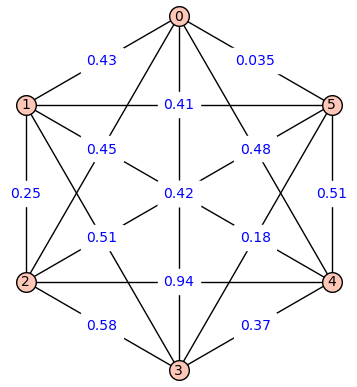
\includegraphics[scale=0.5]{graf1}
    \centering
\end{figure}

Končno pa sva s pomočjo \emph{SageMath-a} napisali še \textbf{celoštevilski linearni program}, 
ki vrne pare vozlišč, med katerimi so povezave v najcenejšem prirejanju $M,$ vsoto cen povezav v $M$ 
in nariše graf z označenimi povezavami, ki so v najcenejšem prirejanju.

\small
\begin{verbatim}
def clp(G):
    p = MixedIntegerLinearProgram(maximization=False)
    b = p.new_variable(binary=True)
    p.set_objective(sum([w * b[Set(e)] for *e, w in G.edges(labels=True)]))

    for v in G:
        p.add_constraint(sum([b[Set(e)] 
                        for e in G.edges_incident(v, labels=False)]) == 1)

    cena = p.solve()
    b = p.get_values(b)

    M = [tuple(e) for e, i in b.items() if i]
    print(M) # pari vozlišč, med katerimi so povezave v najcenejšem prirejanju

    x = [w for *e, w in G.edges() if tuple(e) in M] # seznam cen povezav v M
    print(sum(x)) # vsota cen povezav v M

    H = Graph([(*e, N(w, digits=2)) for *e, w in G.edges(labels=True)])
    H.set_pos(G.get_pos())

    return H.plot(edge_colors={"red": M}, edge_labels=True) 
    # graf H z rdeče pobarvanimi povezavami iz prirejanja
\end{verbatim}
\normalsize

Ko na generiranem grafu želimo najti povezave v najcenejšem prirejanju z uporabo funkcije \texttt{clp} dobimo
seznam parov vozlišč, med katerimi so povezave v najcenejšem prirejanju: \texttt{$[(0, 5), (1, 2), (3, 4)]$} in skupno vsoto cen teh povezav $0.6531541582221374$ (slika \ref{fig:graf1clp}).

\begin{figure}[h!]
    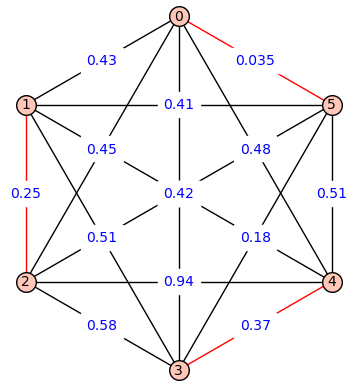
\includegraphics[scale=0.5]{graf1clp}
    \centering
    \caption{Graf z označenimi povezavami, ki so v najcenejšem prirejanju}
    \label{fig:graf1clp}
\end{figure}

\subsection{Analiza rezultatov}
Celoštevilski linearnih program sva večkrat pognali na generiranih grafih, dobljene skupne vsote cen povezav v najnižjem prirejanju pa sva izpisovali v \texttt{.csv} datoteko za lažji uvoz in obdelavo v programskem jeziku \emph{R.}
Nato sva iz vektorja večih ponovitev izračunali njegovo povprečje za posamezen $n$.
Najprej naju je zanimalo, kaj se dogaja s pričakovano vrednostjo najcenejšega prirejanja v polnem grafu, ko točke izberemo enakomerno v enotskem kvadratu.

\begin{figure}[h!]
    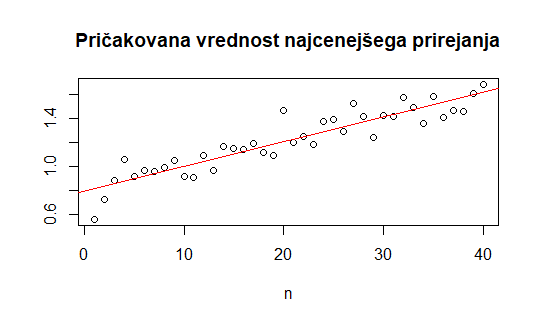
\includegraphics[scale=0.6]{pricak_vred_n_od_1_do_40}
    \centering
    \caption{Graf pričakovane vrednosti najcenejšega prirejanja v odvisnosti od $n$, za $n=1,2,\ldots,40$.}
    \label{fig:pv1-40}
\end{figure}

Na grafu \ref{fig:pv1-40} lahko vidimo, da se z $n$ povečujejo tudi pričakovane vrednosti najcenejših prirejanj.
Zanimivo sa nama je zdelo predvsem, da po začetnem linearnem naraščanju pri $n=1,2,3$ in $4,$ pričakovana vrednost pade, preden začne spet naraščati.
Pade spet pri $n=10$ in še nekajkrat za večje $n.$
Odstopanja od linearnosti sva pripisali malemu številu ponovitev (zaradi počasnosti algoritma sva CLP pognali 10-krat), sva pa se odločili za nizke $n=3,4,5$ algoritem ponoviti dvestokrat.

\begin{figure}[!htb]
    \minipage{0.5\textwidth}
      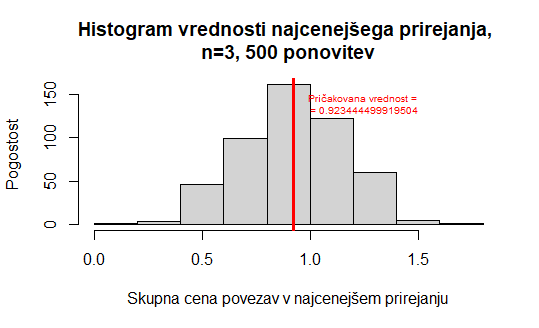
\includegraphics[width=\linewidth]{pricak_vred_n_3.png}
    \endminipage\hfill
    \minipage{0.5\textwidth}
      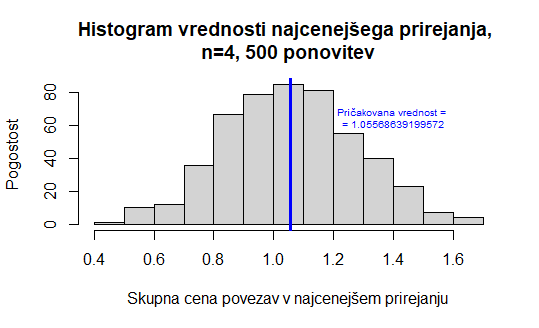
\includegraphics[width=\linewidth]{pricak_vred_n_4.png}
    \endminipage\hfill
\end{figure}

\begin{figure}[!htb]
    \minipage{0.5\textwidth}
      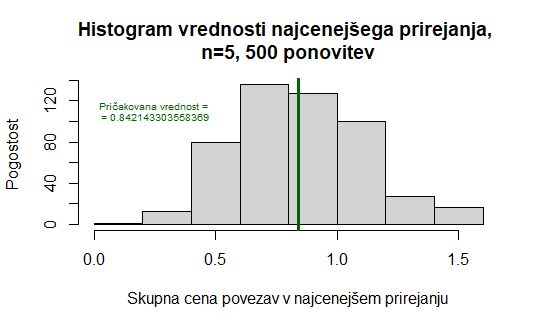
\includegraphics[width=\linewidth]{pricak_vred_n_5.png}
    \endminipage\hfill
    \centering
\end{figure}

Kot je razvidno iz histogramov, se z $n=3$ na $n=4$ pričakovana vrednost skladno z linearnostjo poveča, pri $n=5$ pa tudi pri $200$ ponovitvah zmanjša.

\subsubsection*{Izbira točk in norme}
Pri generiranju grafov sva lahko izbirali med grafi, ki izberejo točke enakomerno v enotskem kvadratu, enotskem krogu in enakostraničnem trikotniku.
\begin{figure}[!htb]
    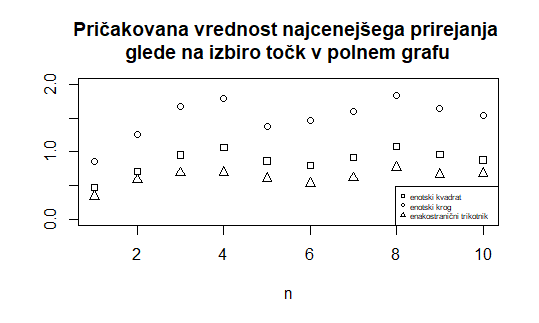
\includegraphics[scale=0.5]{izbira_tock_polni}
    \centering
    \caption{Primerjava pričakovanih vrednosti cene najcenejšega prirejanja glede na izbiro točk}
    \label{fig:tocke}
\end{figure}

S slike \ref{fig:tocke} je lepo razvidno, da je cena povezav (za n od $1$ do $10$) v prirejanju najnižja, ko jih izberemo v enakostraničnem trikotniku in najvišja, ko jih izberemo v enotskem krogu.

V funkcijo za generiranje grafov oziroma natančneje za izračun dolžin med točkami, tj. cen povezav, sva uvedli tudi možnost izračuna z različnimi normami.
Na sliki \ref{fig:norme} vidimo, da bo popolno prirejanje imelo najnižjo ceno, če razdaljo med točkami računamo z neskončno normo in najvišjo, če jo računamo z 1-normo.

\begin{figure}[!htb]
    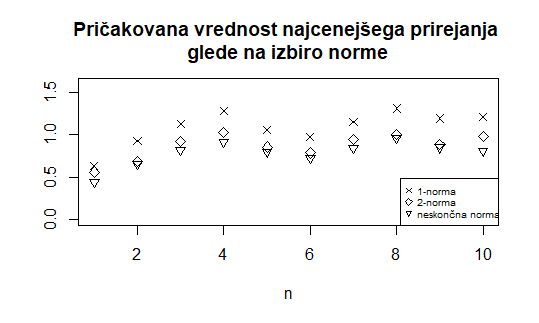
\includegraphics[scale=0.6]{izbira_norme}
    \centering
    \caption{Primerjava pričakovanih vrednosti cene najcenejšega prirejanja glede na izbiro norme}
    \label{fig:norme}
\end{figure}

\subsubsection*{Časovna zahtevnost algoritma}
Časovna zahtevnost algoritma, ki vrne najcenejše prirejanje, je v najinem primeru \emph{eksponentna}.
Za večje $n$ je bilo vedno zahtevneje najti prirejanje z najnižjo ceno, zato sva pričakovane vrednosti poiskali za graf z največ $80$ vozlišči ($n=40$).

\begin{figure}[h!]
    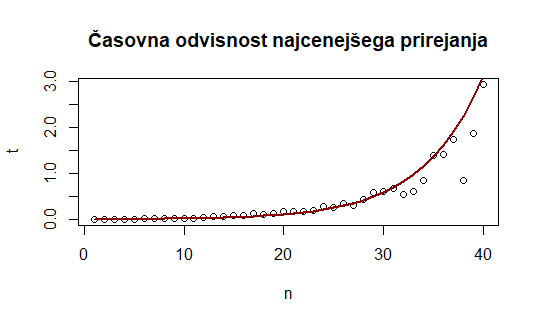
\includegraphics[scale=0.7]{cas_odv_polni}
    \centering
\end{figure}

\section{Dvobarvno najcenejše prirejanje}
\subsection{Opis problema}
Množico $P$ sestavljata množica $n$ rdečih točk, $R,$ in množica $n$ modrih točk $B,$ $P=R \cup B.$
V tem primeru je $G(P,E)$ dvodelen graf z lastnostjo, da med dvema točkama obstaja povezava, če in samo če sta različnih barv.
Cene povezav $(u,v)$ so tako kot v osnovnem primeru razdalje med vozlišči, $d(u,v).$
Spet iščemo najcenejše popolno prirejanje in njegovo ceno.

\subsection{Programiranje rešitev in eksperimentiranje}
Za programiranje rešitev sva ponovno uporabili \emph{SageMath.} Napisali sva funkcijo \texttt{dvobarven\underline{\space}graf,} ki je precej podobna prvotni funkciji,
razlikuje se predvsem v tem, da graf izdela s funkcijo \texttt{CompleteBipartiteGraph(n, n)}.
Za iskanje najcenejšega prirejanja sva uporabili enak celoštevilski linearni program.

\begin{figure}[!htb]
    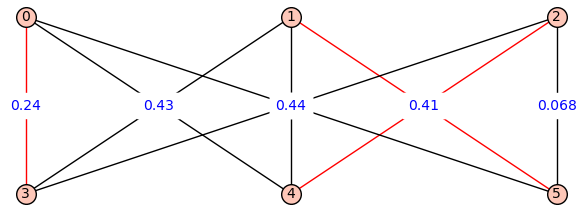
\includegraphics[scale=0.5]{dvobarvenclp}
    \centering
    \caption{Rešen problem najcenejšega prirejanja na dvobarvnem grafu, ko točke izberemo naključno v enakostraničnem trikotniku in za računanje razdalje med njimi uporabimo neskončno normo.}
    \label{fig:dvobarvenclp}
\end{figure}

\subsection{Analiza rezultatov}
Kot je razvidno s spodnje slike, tudi v dvodelnem grafu pričakovana vrednost najcenejšega prirejanja narašča, vendar pa ne narašča enako hitro kot v polnem grafu.
Že pri $n=12$ je razlika v skupni ceni, ko točke izberemo na enotskem kvadratu, večja od ene enote.
\begin{figure}[!htb]
    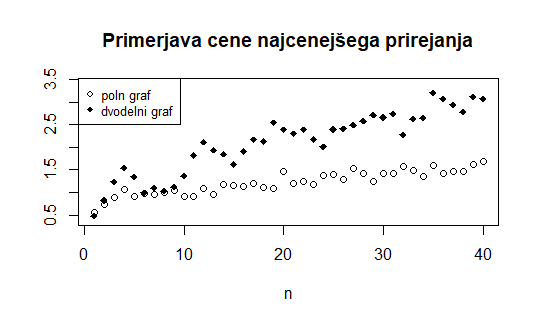
\includegraphics[scale=0.5]{primerjava_cene_polni_dvodelni}
    \centering
\end{figure}

Pri \textbf{časovni odvisnosti} algoritma lahko vidimo, da v dvodelnem grafu najcenejše prirejanje najdemo veliko hitreje kot v polnem.
Razlika je vse bolj očitna z večanjem števila vozlišč. 
Temu je verjetno tako, ker ima dvobarvni graf manj povezav, ki bi jih moral CLP upoštevati pri iskanju prirejanja.

\begin{figure}[!htb]
    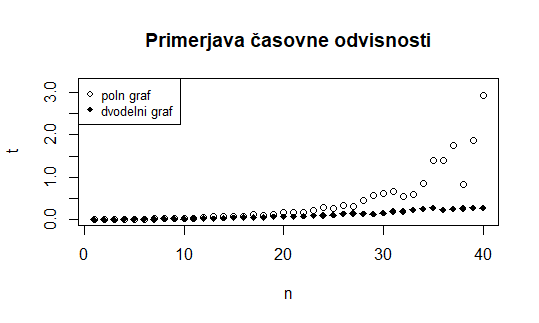
\includegraphics[scale=0.65]{primerjava_cas_polni_dvodelni}
    \centering
\end{figure}

\end{document}